We have already examined the case of generating a subgroup with one element ($<x>)$. What does it mean to generate a subgroup or a group with more than one element?

\begin{example}
    $D_{2n} = $ symmetries of a regular n-gon centered around the origin. Let $r$ be a $360/n$ clockwise rotation of the n-gon about the origin. Let $S$ be a reflection of the n-gon about the line from vertex $1$ to the origin.

    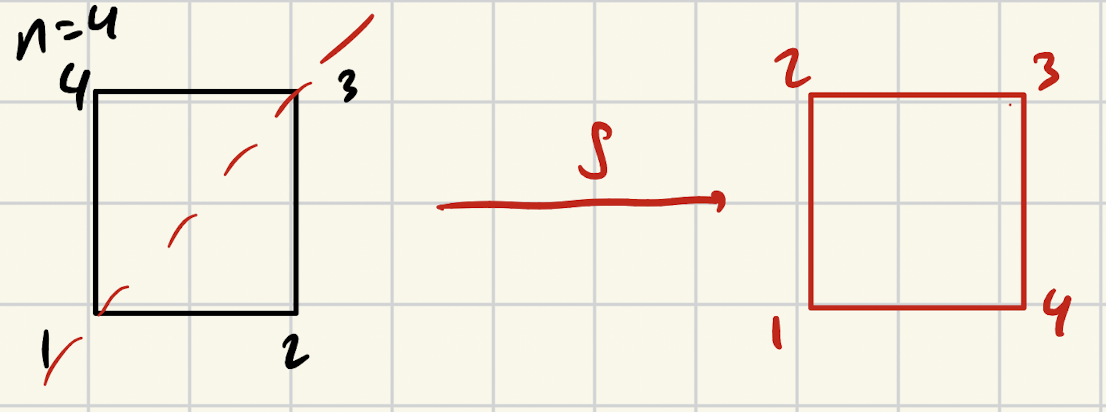
\includegraphics[width= 100pt, center]{/Users/josiahvillarante/GradSchool/Grad-School-Notes/Math210A/CH2/images/Symmetry over vertex 1.png}

    Notice: $1, r, r^2, r^3$ are all distinct. Now consider $s, sr, sr^2, sr^3$ (we read these right-to-left). $sr^3$ is the $270^\circ$ rotation clockwise, then the reflection about the line where vertex $1$ was to the origin.

    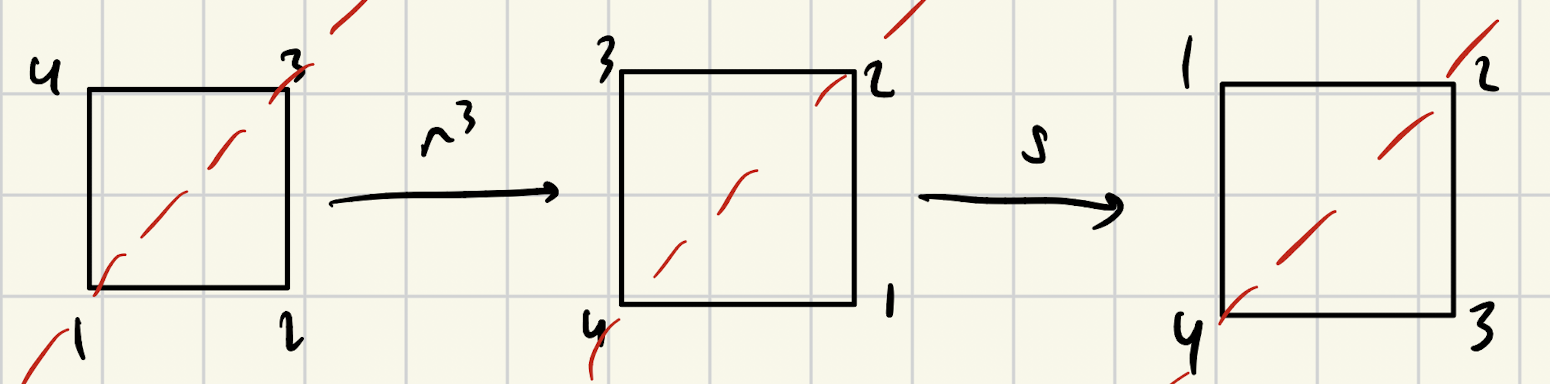
\includegraphics[width= 100pt, center]{/Users/josiahvillarante/GradSchool/Grad-School-Notes/Math210A/CH2/images/sr^3.png}

    Is $s \in \set{1, r, r^2, r^3}?$ No, $s$ fixes vertex $1$ and the only element that fixes vertex $1$ is the identity. But $s \not = 1$, so $s$ is not a rotation. From here, we can deduce that
    $$sr^j \not r^i$$
    for any $0 \leq j \leq 3$ or $0 \leq i \leq 3$ (if it were true that $sr^j = r^i$ for some $i$ and $j$, then $s = r^{i-j}$). Hence $D_{2\dot 4} = \set{1, r, r^2, r^3, s, sr, sr^2, sr^3} = <r, s>/$
\end{example}

In $D_{2n}, n \geq 3,$ we want to show that 
$$D_{2n} = \set{e, r, r^2, r^3, ..., r^{n-1}, s, sr, sr^2, ..., sr^{n-1}}$$
where $s$ is a reflection over the line passing through vertex $1$ and the origin.

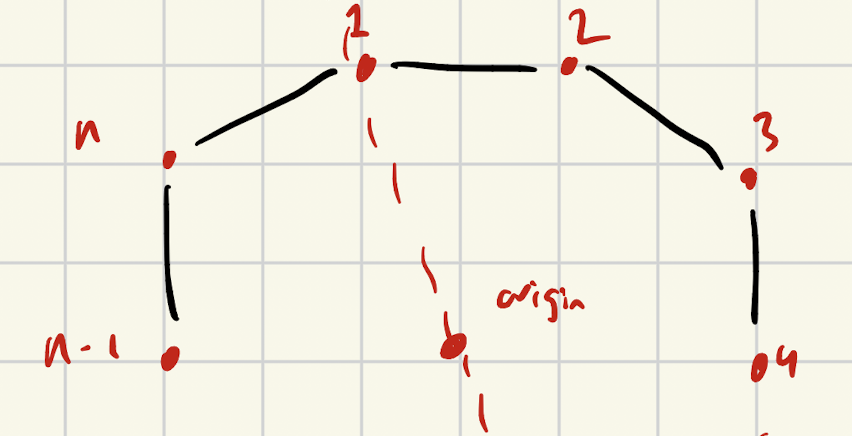
\includegraphics[width= 100pt, center]{/Users/josiahvillarante/GradSchool/Grad-School-Notes/Math210A/CH2/images/n-gon reflection.png}

\begin{enumerate}
    \item Why are all $e, r, r^2, ..., r^{n-1}$ distinct? 
    \begin{align*}
        r^i(1) &= i + 1 \text{ for $0\leq i \leq n -1$ } \\
        r^i(1) &= r^j(1) \\
        \implies i + 1 &= j + 1 \\
        \implies i &= j
    \end{align*}
    so the $r^i$'s are distinct.

    \item $s \not = r^i$ for any $i \in \set{0, ..., n-1}$. $s(1) = 1$ if $r^i(1) = 1,$ we know from part 1 that $i = 0$. That is, $r^i = e$. But $s(2) = n \not = 2 = e(2) \implies s \not = e, s \not = r^i ~\forall 0 \leq i \leq n$

    \item Let's show that $r^i \not = sr^j$ for any $i, j \in \set{0, ..., n-1} = A$.
    Suppose there exists $i,j\in A \st r^i = sr^j$. We define $r^{-1}$ as a counter-clockwise rotation; $r^-1 = r^{n-1}$. This gives 
    \begin{align*}
        r^i &= sr^j \\
        \implies r^{i-j} &= s \\
        \implies r^{i + n-j} &= s
    \end{align*}
    where we adjust $(i + n-j) \mod n$ as needed. This contradicts $s \not \in \set{e, r, r^2, ..., r^{n-1}}$. Hence $r^i \not = sr^j$ for any $i, j \in A$.

    \item Show that $sr^i \not = sr^j$ for any $i \not = j$ in $A$.
    For the sake of contradiction, suppose there exists $i, j \in A \st sr^i = sr^j.$ Then 
    \begin{align*}
        s^2r^i &= s^2r^j \\
        \implies er^i &= er^j \\
        \implies r^i &= r^j
    \end{align*}
    This contradicts $i \not = j$.
    \begin{align*}
        &D_{2n} = \set{e, r, r^2, ..., r^{n-1}, s, sr, sr^2, ..., sr^{n-1}} \\ 
        &sr \not = rs \\
        (s\circ r)(1)=s(r(1)) &&(r \circ s)(1)=r(s(1)) \\
        = s(2)  &&= r(1)  \\
        = n  &&= 2
    \end{align*}
    But $sr = r^{-1}s$. If $sr(1) = r^{-1}s(1)$ and $sr(2) = r^{-1}s(2),$ then $sr = r^{-1}s.$ It can be shown inductively that $sr^i = r^{-i}s ~\forall i \in \Z.$
\end{enumerate}

Let $ x\in G$ and $H \leq G$. If $x \in H$, then $<x> \leq H$. In some sense, $<x>$ is the smallest subgroup of $G$ which contains $x$. "Smallest" refers to containment.

\begin{proposition}
    \label{prop8}
    If $\mathcal{A}$ is any collection of subgrops of a group $G$, then $\bigcap \limits_{H \in \mathcal{A}} H \leq G.$
\end{proposition}

\begin{proof}
    HW
\end{proof}

\begin{definition}[Generating Sets] \leavevmode \\
    If $A$ is any subset of the group $G$, define
    $$<A> = \bigcap \limits_{H \leq G, A \subseteq H} H$$
    This is called the subgroup of $G$ generated by $A$. $A$ is called the generating set. 
\end{definition}

Notice that in the notation of prop \ref{prop8}
$$\mathcal{A} = \set{H \leq G : A \subseteq H} \text{(nonempty as $G \in A$ since $G\leq G$ and $A \subseteq G$)}$$
We will show that $<A> $ is the unique minimal element of $\mathcal{A}$.

We know that $A \subseteq H ~~\forall H \in \mathcal{A}.$ Thus $A \subseteq <A>, $ so $<A> \in \mathcal{A}$.
Let $K \in \mathcal{A}.$ We know that 
$$\bigcap \limits_{H\in \mathcal{A}} H \leq K$$
That is, $<A> \leq K.$ Hence, $<A>$ is minimal with respect to inclusion. When $A$ is finite, that is
$$A = \set{a_1, ..., a_n} \text{ for } n \in \N$$
then we write 
$$<A> = <a_1, a_2, ..., a_n>$$
This is a more concrete verion of the previous set $<A> = \bigcap \limits_{H \leq G, A \subseteq H} H.$
Denote
$$\overline{A} = \set{a_1^{\epsilon_1} a_2^{\epsilon_2} ... a_n^{\epsilon_n} : n \in \N, \epsilon_i = \pm 1, a_i \in A}$$

In $D_{2n}$, $x \in <r,s>$ could look like
$$rssssssr^{-1}s^{-1}srrs^{-1}rr^{-1}s = r^2$$

\begin{proposition}
    $<A> = \overline{A}$.
\end{proposition}